% ============================================================
%  CHAPITRE : PROBABILITÉS
%  Mazava Maths — Terminale S (Bacc Série S, Madagascar)
%  Aligné sur le modèle type et le programme officiel MESUPRES
%  (vocabulaire ; équiprobabilité ; dénombrement : principe
%  multiplicatif, p-listes, arrangements, permutations,
%  combinaisons ; événement contraire ; réunion : incompatibles
%  et cas général — formule de Poincaré ; système complet).
%  Environnements : definition, propriete, theoreme, methode,
%                   attention, astucebac, exemple, exercice,
%                   solution, remarque
% ============================================================
\chapter{Probabilités}

\begin{citationchapitre}
	« La théorie des probabilités n'est au fond que le bon sens réduit
	au calcul. »\\[0.4em]
	— Pierre-Simon de Laplace
\end{citationchapitre}

\begin{objectifs}
	\begin{itemize}[label=\textbullet]
		\item Maîtriser le vocabulaire des probabilités : univers, issue,
		événement, événements incompatibles, système complet.
		\item Calculer une probabilité dans une situation d'\textbf{équiprobabilité}
		et dans un modèle donné par une loi.
		\item \textbf{Dénombrer} : principe multiplicatif, $p$-listes,
		arrangements, permutations, combinaisons.
		\item Utiliser la probabilité de l'\textbf{événement contraire}
		($\Prob(\overline{A})=1-\Prob(A)$).
		\item Calculer $\Prob(A\cup B)$ pour des événements incompatibles et
		dans le cas général (\textbf{formule de Poincaré}).
	\end{itemize}
\end{objectifs}


% ============================================================
\section{Vocabulaire des probabilités}
% ============================================================

\begin{definition}[Expérience aléatoire]
	Une \textbf{expérience aléatoire} est une expérience dont on ne peut pas
	prévoir le résultat avec certitude, mais dont on connaît à l'avance
	l'ensemble des résultats possibles.

	Cet ensemble des résultats possibles s'appelle l'\textbf{univers} de
	l'expérience, noté $\Omega$. Chaque élément de $\Omega$ est une
	\textbf{issue} (ou \textbf{éventualité}).
\end{definition}

\begin{exemple}
	On lance un dé cubique équilibré. L'univers est $\Omega = \{1,2,3,4,5,6\}$.
	Chaque résultat (« obtenir $3$ », par exemple) est une issue.
\end{exemple}

\begin{definition}[Événement]
	Un \textbf{événement} est une partie (un sous-ensemble) de $\Omega$.
	\begin{itemize}[label=\textbullet]
		\item Un \textbf{événement élémentaire} est un événement réduit à une
		seule issue $\{\omega\}$.
		\item L'\textbf{événement certain} est l'univers $\Omega$ tout entier :
		il est toujours réalisé.
		\item L'\textbf{événement impossible} est l'ensemble vide $\emptyset$ :
		il n'est jamais réalisé.
	\end{itemize}
\end{definition}

\begin{center}
	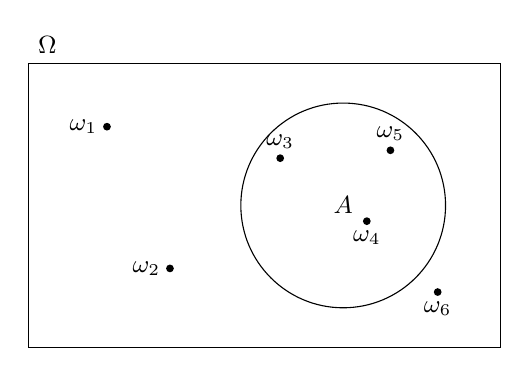
\begin{tikzpicture}[>=stealth, font=\small]
		\draw (0,0) rectangle (6,3.6);
		\node[above right] at (0,3.6) {$\Omega$};
		\draw (4,1.8) circle (1.3);
		\node at (4,1.8) {$A$};
		\foreach \p/\lab in {{(1,2.8)/1},{(1.8,1)/2},{(3.2,2.4)/3},{(4.3,1.6)/4},{(4.6,2.5)/5},{(5.2,0.7)/6}}{
			\fill[black] \p circle (1.4pt);
		}
		\node[left] at (1,2.8) {$\omega_1$};
		\node[left] at (1.8,1) {$\omega_2$};
		\node[above] at (3.2,2.4) {$\omega_3$};
		\node[below] at (4.3,1.6) {$\omega_4$};
		\node[above] at (4.6,2.5) {$\omega_5$};
		\node[below] at (5.2,0.7) {$\omega_6$};
	\end{tikzpicture}
\end{center}

\begin{definition}[Opérations sur les événements]
	Soient $A$ et $B$ deux événements de $\Omega$.
	\begin{itemize}[label=\textbullet]
		\item $A\cap B$ (« $A$ \textbf{et} $B$ ») est l'événement réalisé
		lorsque $A$ et $B$ le sont tous les deux.
		\item $A\cup B$ (« $A$ \textbf{ou} $B$ ») est réalisé lorsque l'un au
		moins de $A$, $B$ l'est.
		\item $\overline{A}$ (« \textbf{non} $A$ ») est réalisé lorsque $A$ ne
		l'est pas.
	\end{itemize}
	$A$ et $B$ sont \textbf{incompatibles} lorsque $A\cap B=\emptyset$.
\end{definition}

\begin{definition}[Système complet d'événements]
	Les événements $A_1,A_2,\ldots,A_n$ forment un \textbf{système complet}
	(ou une \textbf{partition}) de $\Omega$ lorsqu'ils sont deux à deux
	incompatibles et que leur réunion est $\Omega$ : toute issue appartient à
	un $A_i$ et à un seul. En particulier, $A$ et $\overline{A}$ forment
	toujours un système complet.
\end{definition}


% ============================================================
\section{Probabilité d'un événement}
% ============================================================

\begin{definition}[Probabilité]
	Définir une \textbf{probabilité} sur $\Omega$, c'est associer à chaque
	issue $\omega_i$ un nombre $p_i \in [0\,;1]$, appelé \textbf{probabilité}
	de $\omega_i$, tel que la somme de tous les $p_i$ soit égale à $1$.

	La probabilité d'un événement $A$, notée $\Prob(A)$, est la somme des
	probabilités des issues qui le composent.
\end{definition}

\begin{propriete}{Propriétés immédiates}{prop_proba_base}
	\begin{itemize}[label=\textbullet]
		\item $\Prob(\emptyset) = 0$ et $\Prob(\Omega) = 1$.
		\item Pour tout événement $A$ : $0 \leqslant \Prob(A) \leqslant 1$.
		\item Si $A\subset B$, alors $\Prob(A)\leqslant\Prob(B)$.
		\item Si $A_1,\ldots,A_n$ forment un système complet, alors
		$\Prob(A_1)+\cdots+\Prob(A_n)=1$.
	\end{itemize}
\end{propriete}

\begin{definition}[Situation d'équiprobabilité]
	On dit qu'il y a \textbf{équiprobabilité} lorsque toutes les issues de
	$\Omega$ ont la même probabilité. Dans ce cas, pour tout événement $A$ :
	\[
	\Prob(A) = \frac{\mathrm{card}(A)}{\mathrm{card}(\Omega)}
	= \frac{\text{nombre de cas favorables à } A}{\text{nombre de cas possibles}}.
	\]
\end{definition}

\begin{exemple}
	On tire au hasard une carte dans un jeu de $32$ cartes. Soit $A$ : « la
	carte tirée est un roi ». On a $\mathrm{card}(\Omega)=32$ et
	$\mathrm{card}(A)=4$, donc $\Prob(A) = \dfrac{4}{32} = \dfrac{1}{8}$.
\end{exemple}

\begin{astucebac}
	Reconnaître l'équiprobabilité : dé non pipé, pièce équilibrée, boules
	\emph{indiscernables au toucher}, carte tirée \emph{au hasard}, choix
	\emph{au hasard} d'une personne dans un groupe. Si l'énoncé donne un dé
	\emph{pipé} ou des probabilités inégales, on travaille directement avec la
	loi $(p_i)$.
\end{astucebac}


% ============================================================
\section{Dénombrement}
% ============================================================

En situation d'équiprobabilité, calculer une probabilité revient à
\textbf{compter} : $\mathrm{card}(\Omega)$ et $\mathrm{card}(A)$.

\begin{propriete}{Principe multiplicatif}{prop_mult}
	Si une expérience se déroule en $k$ étapes successives, offrant
	respectivement $n_1, n_2, \ldots, n_k$ possibilités (le nombre de
	possibilités d'une étape ne dépendant pas des choix précédents), alors le
	nombre total de résultats est
	\[
	n_1\times n_2\times\cdots\times n_k.
	\]
\end{propriete}

\begin{exemple}
	Un code est formé de $2$ lettres (parmi $26$) suivies de $3$ chiffres
	(parmi $10$). Il y a $26^2\times 10^3 = 676\,000$ codes possibles.
\end{exemple}

\begin{definition}[Factorielle]
	Pour $n\in\N^*$, on pose $n! = 1\times 2\times\cdots\times n$, et $0!=1$.
\end{definition}

\begin{theoreme}[Trois modèles de tirage de $p$ objets parmi $n$]
	\begin{center}
	\renewcommand{\arraystretch}{2.2}
	\begin{tabular}{>{\raggedright\arraybackslash}p{3.5cm}
	                >{\centering\arraybackslash}p{2.6cm}
	                >{\centering\arraybackslash}p{3.4cm}}
	\hline
	\textbf{Modèle} & \textbf{Ordre} & \textbf{Nombre} \\
	\hline
	$p$-liste (tirages successifs \emph{avec} remise) & compte &
	$n^{p}$ \\
	Arrangement (successifs \emph{sans} remise) & compte &
	$A_n^{p}=\dfrac{n!}{(n-p)!}$ \\
	Permutation ($p=n$, sans remise) & compte & $n!$ \\
	Combinaison (tirage \emph{simultané}) & ne compte pas &
	$\dbinom{n}{p}=\dfrac{n!}{p!\,(n-p)!}$ \\
	\hline
	\end{tabular}
	\end{center}
\end{theoreme}

\begin{propriete}{Coefficients binomiaux}{prop_binom_proba}
	Pour $0\leqslant p\leqslant n$ :
	\[
	\binom{n}{0}=\binom{n}{n}=1,\qquad
	\binom{n}{p}=\binom{n}{n-p},\qquad
	\binom{n}{p-1}+\binom{n}{p}=\binom{n+1}{p}.
	\]
\end{propriete}

\begin{methode}
	\textbf{Choisir le bon modèle :}
	\begin{enumerate}
		\item L'ordre des objets tirés intervient-il ? (podium, code, mot :
		oui ; poignée de jetons, comité, main de cartes : non).
		\item Un même objet peut-il être choisi plusieurs fois ? (avec remise :
		oui ; sans remise / simultané : non).
		\item En déduire : $n^p$, $A_n^p$, $n!$ ou $\dbinom{n}{p}$.
	\end{enumerate}
\end{methode}

\begin{exemple}
	Une urne contient $10$ jetons numérotés. On en tire $3$ \emph{simultanément}
	: il y a $\dbinom{10}{3}=\dfrac{10\times 9\times 8}{3!}=120$ tirages
	possibles. Si l'on tire les $3$ jetons \emph{l'un après l'autre sans
	remise}, il y en a $A_{10}^{3}=10\times 9\times 8 = 720$.
\end{exemple}


% ============================================================
\section{Événement contraire, réunion}
% ============================================================

\begin{center}
	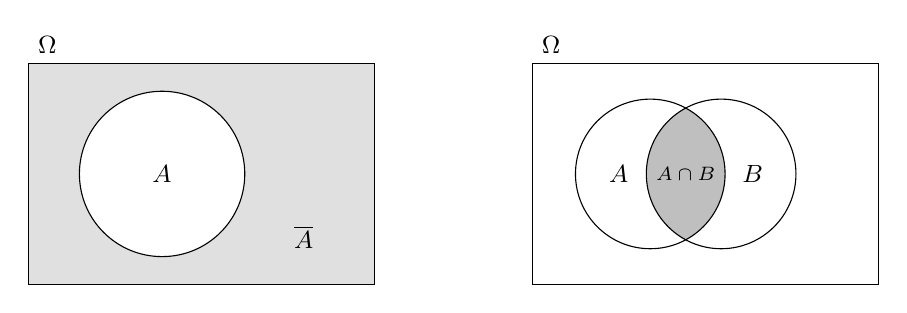
\begin{tikzpicture}[>=stealth, font=\small]
		% contraire
		\fill[black!12] (0,0) rectangle (4.4,2.8);
		\draw (0,0) rectangle (4.4,2.8);
		\node[above right] at (0,2.8) {$\Omega$};
		\fill[white] (1.7,1.4) circle (1.05);
		\draw (1.7,1.4) circle (1.05);
		\node at (1.7,1.4) {$A$};
		\node at (3.5,0.6) {$\overline{A}$};
		% réunion générale
		\begin{scope}[xshift=6.4cm]
			\draw (0,0) rectangle (4.4,2.8);
			\node[above right] at (0,2.8) {$\Omega$};
			\begin{scope}
				\clip (1.5,1.4) circle (0.95);
				\fill[black!25] (2.4,1.4) circle (0.95);
			\end{scope}
			\draw (1.5,1.4) circle (0.95);
			\draw (2.4,1.4) circle (0.95);
			\node at (1.1,1.4) {$A$};
			\node at (2.8,1.4) {$B$};
			\node at (1.95,1.4) {\scriptsize $A\cap B$};
		\end{scope}
	\end{tikzpicture}
\end{center}

\begin{propriete}{Probabilité de l'événement contraire}{prop_contraire}
	Pour tout événement $A$ : $\Prob(\overline{A}) = 1 - \Prob(A)$.
\end{propriete}

\begin{astucebac}
	Il est souvent plus rapide de passer par l'événement contraire, en
	particulier avec les formulations « \textbf{au moins un}\ldots » :
	\[
	\Prob(\text{« au moins un »}) = 1 - \Prob(\text{« aucun »}).
	\]
\end{astucebac}

\begin{propriete}{Probabilité d'une réunion — formule de Poincaré}{prop_poincare}
	\begin{itemize}[label=\textbullet]
		\item Si $A$ et $B$ sont \textbf{incompatibles} :
		$\Prob(A \cup B) = \Prob(A) + \Prob(B)$.
		\item Dans le \textbf{cas général} :
		\[
		\Prob(A \cup B) = \Prob(A) + \Prob(B) - \Prob(A \cap B).
		\]
	\end{itemize}
\end{propriete}

\begin{exemple}
	On tire une carte dans un jeu de $32$ cartes. Soit $A$ : « tirer un roi »
	et $B$ : « tirer un cœur ». On a $\Prob(A) = \dfrac{4}{32}$,
	$\Prob(B) = \dfrac{8}{32}$ et $\Prob(A\cap B) = \dfrac{1}{32}$ (le roi de
	cœur), donc
	\[
	\Prob(A\cup B) = \frac{4}{32} + \frac{8}{32} - \frac{1}{32} = \frac{11}{32}.
	\]
\end{exemple}

\begin{attention}
	Deux événements \textbf{incompatibles} ($A\cap B=\emptyset$) ne sont pas
	« indépendants » : ce sont deux notions distinctes (voir le chapitre
	suivant).
\end{attention}


% ============================================================
\section{Méthodes et exercices résolus}
% ============================================================

\begin{methode}
	\textbf{Calculer une probabilité en situation d'équiprobabilité :}
	\begin{enumerate}
		\item décrire l'expérience et justifier l'équiprobabilité ;
		\item choisir un modèle de dénombrement et calculer
		$\mathrm{card}(\Omega)$ ;
		\item traduire l'événement, dénombrer $\mathrm{card}(A)$ (au besoin en
		le découpant en cas incompatibles, ou en passant au contraire) ;
		\item conclure : $\Prob(A)=\dfrac{\mathrm{card}(A)}{\mathrm{card}(\Omega)}$.
	\end{enumerate}
\end{methode}

\exerciceresolu
\textbf{Tirage simultané dans une urne}

Une urne contient $10$ jetons indiscernables au toucher : $3$ rouges,
$5$ verts et $2$ bleus. On tire simultanément $3$ jetons.
\begin{enumerate}
	\item Déterminer le nombre de tirages possibles.
	\item Calculer la probabilité de tirer $3$ jetons verts.
	\item Calculer la probabilité de tirer exactement $1$ rouge et $2$ verts.
	\item Calculer la probabilité de tirer au moins un bleu.
\end{enumerate}

\solution

\textbf{1.} Un tirage simultané de $3$ jetons parmi $10$ :
$\mathrm{card}(\Omega)=\dbinom{10}{3}=120$.

\textbf{2.} Choisir $3$ verts parmi $5$ : $\dbinom{5}{3}=10$ tirages, donc
$\Prob = \dfrac{10}{120}=\dfrac{1}{12}$.

\textbf{3.} $\dbinom{3}{1}\times\dbinom{5}{2}=3\times 10 = 30$ tirages, donc
$\Prob = \dfrac{30}{120}=\dfrac14$.

\textbf{4.} Contraire : « aucun bleu », soit $3$ jetons parmi les $8$ non
bleus : $\dbinom{8}{3}=56$. Donc
$\Prob(\text{au moins un bleu}) = 1-\dfrac{56}{120}=\dfrac{64}{120}=\dfrac{8}{15}$.

\exerciceresolu
\textbf{Modèle non équiprobable : un dé pipé}

Un dé cubique est truqué de sorte que la probabilité d'obtenir la face $k$
soit proportionnelle à $k$ : $\Prob(\{k\})=k\,a$ pour $k\in\{1,\ldots,6\}$.
\begin{enumerate}
	\item Déterminer $a$.
	\item Calculer la probabilité d'obtenir un nombre pair.
	\item Calculer la probabilité d'obtenir au moins $5$.
\end{enumerate}

\solution

\textbf{1.} La somme des probabilités vaut $1$ :
$a(1+2+3+4+5+6)=21a=1$, donc $a=\dfrac{1}{21}$.

\textbf{2.} « Pair » $=\{2,4,6\}$ :
$\Prob = \dfrac{2+4+6}{21}=\dfrac{12}{21}=\dfrac47$.

\textbf{3.} « Au moins $5$ » $=\{5,6\}$ :
$\Prob = \dfrac{5+6}{21}=\dfrac{11}{21}$.

\exerciceresolu
\textbf{Formule de Poincaré}

Dans une classe de $30$ élèves, $18$ étudient l'anglais, $15$ l'allemand et
$7$ les deux langues. On choisit un élève au hasard.
\begin{enumerate}
	\item Calculer la probabilité qu'il étudie au moins une des deux langues.
	\item Calculer la probabilité qu'il n'étudie aucune de ces deux langues.
	\item Calculer la probabilité qu'il étudie l'anglais mais pas l'allemand.
\end{enumerate}

\solution

Soit $A$ : « étudie l'anglais », $B$ : « étudie l'allemand ». Équiprobabilité
sur les $30$ élèves : $\Prob(A)=\dfrac{18}{30}$, $\Prob(B)=\dfrac{15}{30}$,
$\Prob(A\cap B)=\dfrac{7}{30}$.

\textbf{1.} $\Prob(A\cup B)=\dfrac{18}{30}+\dfrac{15}{30}-\dfrac{7}{30}
=\dfrac{26}{30}=\dfrac{13}{15}$.

\textbf{2.} $\Prob(\overline{A\cup B})=1-\dfrac{13}{15}=\dfrac{2}{15}$
($2$ élèves).

\textbf{3.} $\Prob(A\cap\overline{B})=\Prob(A)-\Prob(A\cap B)
=\dfrac{18}{30}-\dfrac{7}{30}=\dfrac{11}{30}$.


% ============================================================
\section{Exercices d'entraînement}
% ============================================================

% --------------------------------------------------
\subsection{Échauffement}
% --------------------------------------------------

\exercice{Lire une situation \hfill \facile}
On lance un dé cubique équilibré dont les faces sont numérotées de $1$ à $6$.
\begin{enumerate}
	\item Décrire l'univers $\Omega$ de cette expérience.
	\item Décrire par une phrase, puis en extension, l'événement $A$ :
	« obtenir un diviseur de $6$ ».
	\item Donner un événement incompatible avec $A$, puis un système complet
	de deux événements contenant $A$.
	\item Calculer $\Prob(A)$ et $\Prob(\overline{A})$.
\end{enumerate}

\exercice{Diagramme de Venn \hfill \facile}
On interroge $50$ personnes. $30$ possèdent un vélo ($V$), $20$ une moto
($M$), $8$ les deux.
\begin{enumerate}
	\item Reproduire et compléter un diagramme représentant $V$ et $M$.
	\item Combien de personnes ne possèdent ni vélo ni moto ?
	\item Une personne est choisie au hasard : calculer $\Prob(V\cup M)$.
\end{enumerate}

\exercice{Vrai ou faux \hfill \facile}
Répondre par \emph{vrai} ou \emph{faux} en justifiant.
\begin{enumerate}
	\item Si $\Prob(A)=0{,}3$ et $\Prob(B)=0{,}8$, alors $A$ et $B$ ne peuvent
	pas être incompatibles.
	\item On a toujours $\Prob(A\cup B)=\Prob(A)+\Prob(B)$.
	\item Pour tout événement $A$, $\Prob(A)+\Prob(\overline{A})=1$.
	\item Le nombre de mains de $5$ cartes dans un jeu de $32$ est $A_{32}^{5}$.
	\item $\dbinom{7}{2}=\dbinom{7}{5}$.
	\item Tirer successivement $2$ boules \emph{sans remise} et les tirer
	\emph{simultanément} donnent le même nombre de résultats si l'ordre ne
	compte pas.
	\item Si $A$ et $B$ sont incompatibles alors $\overline{A}$ et
	$\overline{B}$ le sont aussi.
\end{enumerate}

% --------------------------------------------------
\subsection{Calculs de probabilités}
% --------------------------------------------------

\exercice{Équiprobabilité directe \hfill \facile}
Une urne contient $4$ boules blanches et $6$ boules noires, indiscernables au
toucher. On tire au hasard une boule.
\begin{multicols}{2}
\begin{enumerate}
	\item Probabilité de tirer une blanche.
	\item Probabilité de tirer une noire (deux méthodes).
	\item On ajoute $2$ boules rouges : nouvelle probabilité de tirer une
	blanche.
	\item Probabilité de ne pas tirer de rouge.
\end{enumerate}
\end{multicols}

\exercice{Deux dés \hfill \moyen}
On lance simultanément deux dés cubiques équilibrés et on note la somme $S$.
\begin{enumerate}
	\item Déterminer $\mathrm{card}(\Omega)$.
	\item Calculer $\Prob(S=7)$, puis $\Prob(S\geqslant 10)$.
	\item En déduire $\Prob(S\leqslant 9)$.
	\item Calculer la probabilité que le produit des deux dés soit pair.
\end{enumerate}

\exercice{Cartes et Poincaré \hfill \moyen}
On tire une carte dans un jeu de $32$ cartes. $A$ : « tirer un as »,
$B$ : « tirer un pique », $C$ : « tirer une figure ».
\begin{multicols}{2}
\begin{enumerate}
	\item $\Prob(A)$, $\Prob(B)$, $\Prob(C)$.
	\item $A$ et $C$ sont-ils incompatibles ?
	\item $\Prob(A\cup B)$.
	\item $\Prob(B\cup C)$.
\end{enumerate}
\end{multicols}

\exercice{Dénombrement \hfill \moyen}
Un club compte $12$ membres : $7$ femmes et $5$ hommes.
\begin{enumerate}
	\item De combien de façons peut-on former un bureau ordonné
	(président, secrétaire, trésorier) ?
	\item De combien de façons peut-on former une délégation de $3$ membres ?
	\item Probabilité que cette délégation soit composée uniquement de femmes.
	\item Probabilité qu'elle comporte au moins un homme.
\end{enumerate}

\exercice{Anagrammes \hfill \difficile}
On considère les mots (ayant un sens ou non) obtenus en permutant les lettres
du mot \textsc{banana}.
\begin{enumerate}
	\item Combien de mots distincts peut-on former ?
	\item On en choisit un au hasard : probabilité qu'il commence par un
	\textsc{b}.
	\item Probabilité que les trois \textsc{a} soient consécutifs.
\end{enumerate}

% --------------------------------------------------
\subsection{Sujets types Bac}
% --------------------------------------------------

\exercice{Sujet type Bac — urne et tirage simultané \hfill \difficile}
Une urne contient $9$ boules indiscernables au toucher : $4$ blanches,
$3$ rouges et $2$ noires. On tire simultanément $3$ boules.

\textbf{Partie A — Dénombrement}
\begin{enumerate}
	\item Justifier qu'il y a $\dbinom{9}{3}=84$ tirages possibles, tous
	équiprobables.
	\item Calculer le nombre de tirages tricolores (une boule de chaque
	couleur).
	\item Calculer le nombre de tirages unicolores.
\end{enumerate}

\textbf{Partie B — Probabilités}
\begin{enumerate}
	\setcounter{enumi}{3}
	\item En déduire $\Prob(T)$ où $T$ : « le tirage est tricolore », puis
	$\Prob(U)$ où $U$ : « le tirage est unicolore ».
	\item Calculer $\Prob(R)$ où $R$ : « le tirage contient au moins une
	rouge » (on pourra passer au contraire).
	\item On note $X$ le nombre de boules blanches obtenues. Déterminer les
	valeurs prises par $X$ et la probabilité $\Prob(X=2)$.
\end{enumerate}

\exercice{Sujet type Bac — un dé pipé \hfill \difficile}
Un dé à six faces est truqué : la probabilité d'obtenir la face $k$ est
$\Prob(\{k\})=\dfrac{k}{21}$ pour $k\in\{1,\ldots,6\}$.
\begin{enumerate}
	\item Vérifier que l'on définit bien une loi de probabilité.
	\item Calculer $\Prob(P)$, $P$ : « obtenir un nombre pair », et
	$\Prob(M)$, $M$ : « obtenir un multiple de $3$ ».
	\item Calculer $\Prob(P\cup M)$ à l'aide de la formule de Poincaré.
	\item On lance ce dé deux fois de suite, les lancers étant indépendants.
	Montrer que la probabilité d'obtenir deux fois un $6$ est
	$\dfrac{36}{441}=\dfrac{4}{49}$.
	\item Calculer la probabilité que la somme des deux lancers soit égale à
	$3$.
\end{enumerate}

\exercice{Sujet type Bac — code d'accès \hfill \difficile}
Un digicode utilise les $10$ chiffres et les lettres \textsc{a} et
\textsc{b}. Un code valide est une suite ordonnée de $4$ symboles.

\textbf{Partie A}
\begin{enumerate}
	\item Combien y a-t-il de codes valides ?
	\item Combien de codes n'utilisent aucune lettre ?
	\item Combien de codes utilisent au moins une lettre ?
\end{enumerate}

\textbf{Partie B}
Un visiteur compose un code au hasard.
\begin{enumerate}
	\setcounter{enumi}{3}
	\item Calculer la probabilité que son code soit formé de $4$ symboles
	distincts.
	\item Calculer la probabilité que son code commence et finisse par un
	chiffre.
	\item Calculer la probabilité qu'il ne contienne que des chiffres pairs.
\end{enumerate}

\exercice{Sujet type Bac — comité mixte \hfill \difficile}
Un conseil est formé de $6$ femmes et $4$ hommes. On choisit au hasard un
comité de $4$ personnes.
\begin{enumerate}
	\item Déterminer le nombre de comités possibles.
	\item Calculer la probabilité que le comité soit composé de $2$ femmes et
	$2$ hommes.
	\item Calculer la probabilité que le comité comporte exactement une femme.
	\item Calculer la probabilité que le comité comporte au moins une femme.
	\item On note $Y$ le nombre de femmes du comité. Recopier et compléter le
	tableau de la loi de $Y$, puis vérifier que la somme des probabilités
	vaut $1$.
\end{enumerate}

\exercice{Sujet type Bac — sondage et formule de Poincaré \hfill \difficile}
On interroge $200$ habitants d'une ville. $120$ lisent le journal $J$,
$90$ écoutent la radio $R$, $50$ font les deux.

\textbf{Partie A}
\begin{enumerate}
	\item Compléter un tableau croisé des effectifs
	($J\cap R$, $J\cap\overline{R}$, $\overline{J}\cap R$,
	$\overline{J}\cap\overline{R}$).
	\item Une personne est choisie au hasard. Calculer $\Prob(J)$,
	$\Prob(R)$, $\Prob(J\cap R)$.
\end{enumerate}

\textbf{Partie B}
\begin{enumerate}
	\setcounter{enumi}{2}
	\item Calculer $\Prob(J\cup R)$ et interpréter.
	\item Calculer la probabilité que la personne ne s'informe ni par $J$ ni
	par $R$.
	\item Calculer la probabilité que la personne s'informe par exactement un
	des deux médias.
\end{enumerate}
